%!TEX root = ./main.tex

\section{What You Already Know}

% SECTION TIMING: 0:00--12:00. Keep all media excerpts short; skip one if discussion runs long.

% Teaching note (60 s): ask students to disable Wi-Fi briefly. Do not interpret
% the icon yet; collect LTE / 5G / 5G UW answers first.
\begin{frame}{What does the icon actually tell you?}
  \begin{columns}[T,onlytextwidth]
    \column{0.39\textwidth}
      \centering
      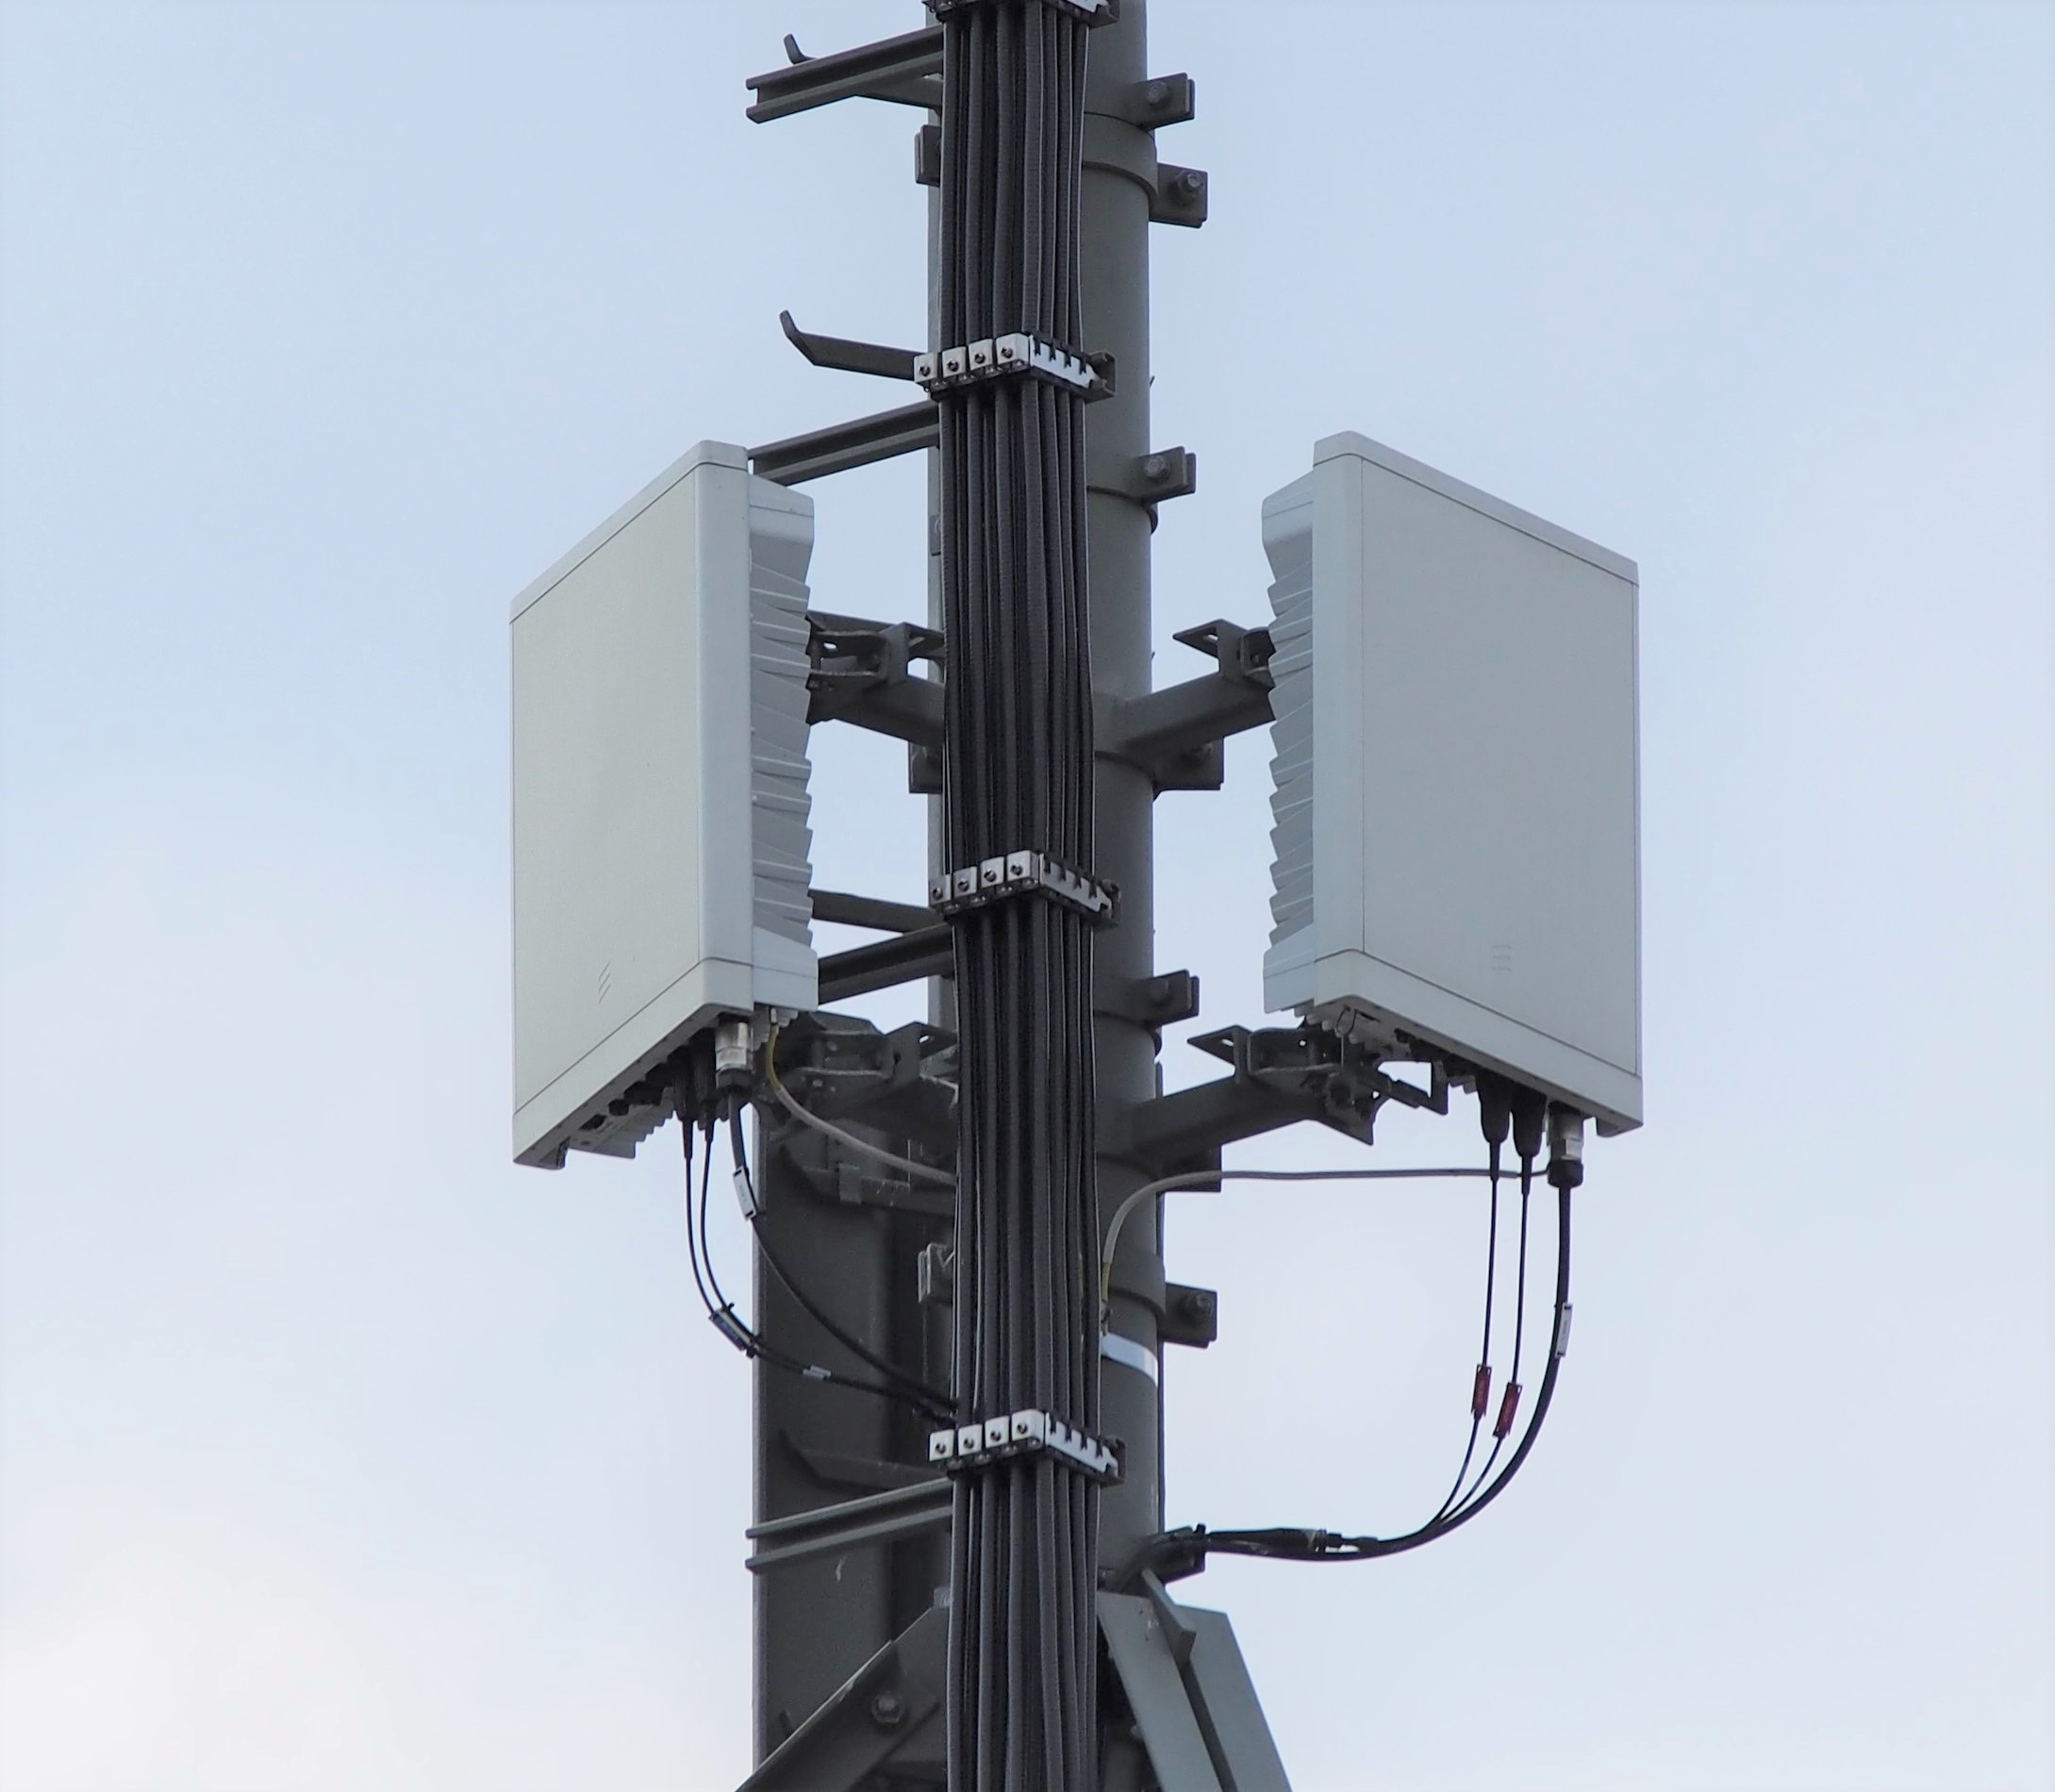
\includegraphics[width=\linewidth]{figure/xg/5g_antenna.jpg}
      \source{https://commons.wikimedia.org/wiki/File:Antennes_actives_5G_Ericsson.jpg}{Ericsson active 5G antennas}
    \column{0.53\textwidth}
      \large\textbf{Turn off Wi-Fi for ten seconds.}

      \vspace{0.7em}
      \normalsize
      What appears: LTE, 5G, 5G+, or 5G UW?

      \vspace{0.8em}
      \ask{Does that icon describe the radio, the core, or the whole network?}
  \end{columns}
\end{frame}

\begin{frame}{Each generation made a new habit feel normal}
  \centering
  \begin{tikzpicture}[
      gen/.style={draw=ranblue,fill=blue!5,rounded corners=3pt,
        minimum width=1.45cm,minimum height=0.75cm,align=center,font=\bfseries},
      note/.style={align=center,font=\scriptsize,text width=1.6cm}
    ]
    \node[gen] (g1) at (0,0) {1G};
    \node[gen] (g2) at (2.1,0) {2G};
    \node[gen] (g3) at (4.2,0) {3G};
    \node[gen] (g4) at (6.3,0) {4G};
    \node[gen] (g5) at (8.4,0) {5G};
    \foreach \a/\b in {g1/g2,g2/g3,g3/g4,g4/g5}
      \draw[flow,draw=ranblue!65] (\a) -- (\b);
    \node[note] at (0,-1.0) {Mobile\\voice};
    \node[note] at (2.1,-1.0) {Text and\\identity};
    \node[note] at (4.2,-1.0) {Mobile\\Internet};
    \node[note] at (6.3,-1.0) {All-IP\\broadband};
    \node[note] at (8.4,-1.0) {Flexible\\systems};
  \end{tikzpicture}

  \vspace{1.1em}
  \Large The app was visible. The architecture underneath was not.
\end{frame}

% Video cue (45 s): first mobile-call story. Play 0:00--0:45.
% https://www.weforum.org/videos/the-first-mobile-phone-call-was-made-50-years-ago/
% Boundary: the 1973 call predates commercial 1G service; it is a doorway into the era.
\begin{frame}{The first mobile call was basically a flex}
  \begin{columns}[T,onlytextwidth]
    \column{0.42\textwidth}
      \centering
      \href{https://www.weforum.org/videos/the-first-mobile-phone-call-was-made-50-years-ago/}{%
        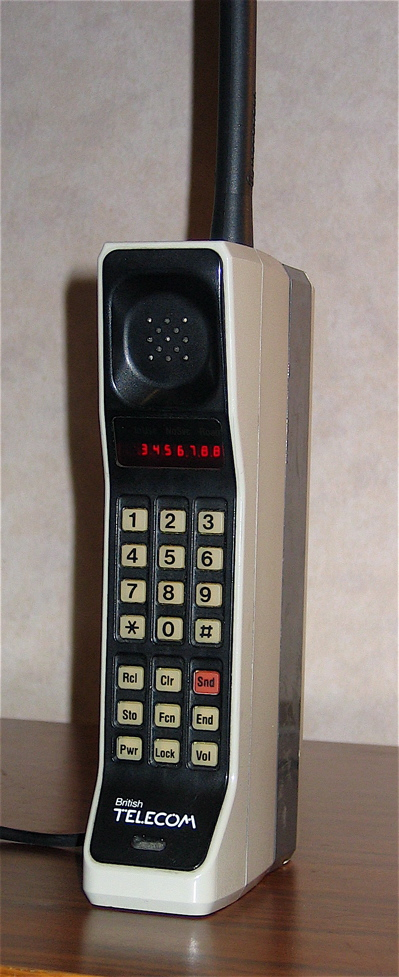
\includegraphics[height=0.65\textheight]{figure/xg/1g_dynatac.jpg}}
      \source{https://commons.wikimedia.org/wiki/File:DynaTAC8000X.jpg}{Motorola DynaTAC 8000X}
    \column{0.58\textwidth}
      \Large\textbf{Martin Cooper called his rival.}

      \vspace{0.7em}
      \normalsize
      \begin{itemize}
        \item The prototype call happened in 1973.
        \item Commercial analog cellular service followed in the 1980s.
        \item The service ordinary users noticed was mobile voice.
      \end{itemize}

      \takeaway{1G moved the telephone away from the wall.}
  \end{columns}
\end{frame}

% Audio cue (25 s): play the familiar Nokia tune. Play 0:00--0:25.
% https://www.youtube.com/watch?v=0F8AmuobbZk
% Boundary: the ringtone is a memory cue, not a 2G standard or launch milestone.
\begin{frame}{The SIM card is the part that knows you}
  \begin{columns}[T,onlytextwidth]
    \column{0.34\textwidth}
      \centering
      \href{https://www.youtube.com/watch?v=0F8AmuobbZk}{%
        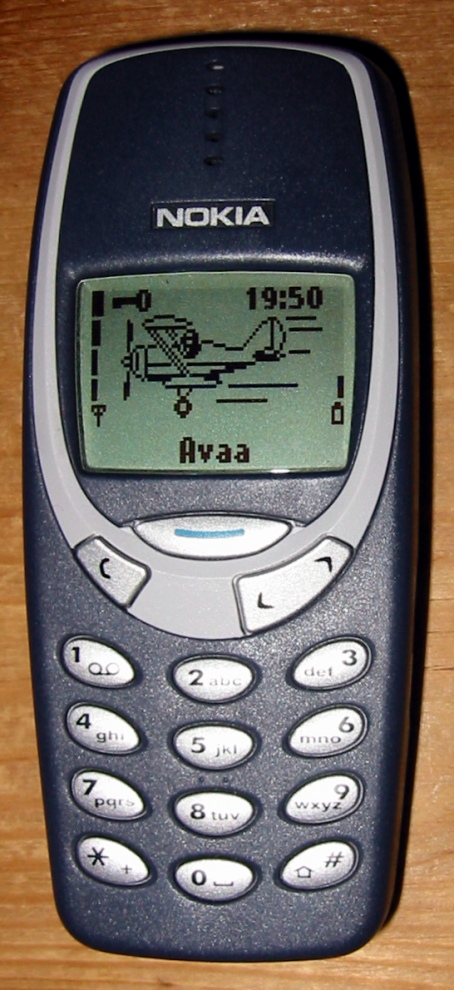
\includegraphics[height=0.57\textheight]{figure/xg/2g_nokia3310.jpg}}
      \source{https://commons.wikimedia.org/wiki/File:Nokia_3310.jpg}{Nokia 3310}
    \column{0.26\textwidth}
      \centering
      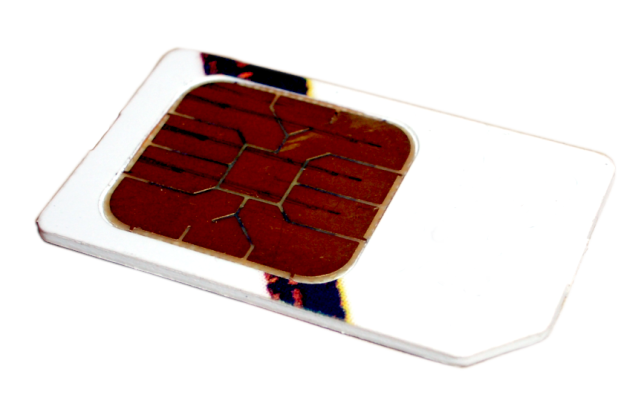
\includegraphics[width=0.95\linewidth]{figure/xg/sim_card.png}
      \source{https://commons.wikimedia.org/wiki/File:Sim_card.png}{GSM SIM card}
    \column{0.40\textwidth}
      \Large\textbf{2G went digital.}
      \normalsize
      \begin{itemize}
        \item Digital voice and SMS
        \item SIM-based subscriber identity in GSM
        \item Mass-market roaming and feature phones
      \end{itemize}
      \ask{Which is ``you'': the phone, the SIM, or the number?}
  \end{columns}
\end{frame}

% Video cue (35 s): Nokia 6680 commercial. Play 0:00--0:35.
% https://www.youtube.com/watch?v=1YAdWbBg0w0
\begin{frame}{3G brought video calls before eye contact}
  \begin{columns}[T,onlytextwidth]
    \column{0.52\textwidth}
      \centering
      \href{https://www.youtube.com/watch?v=1YAdWbBg0w0}{%
        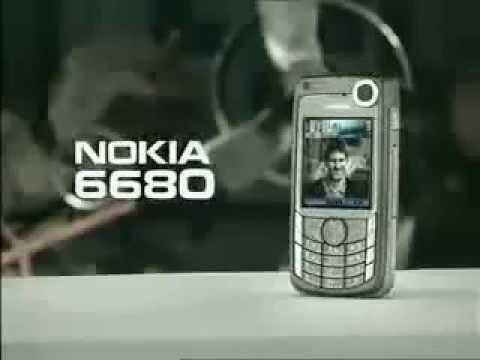
\includegraphics[width=\linewidth]{figure/xg/video_nokia6680.jpg}}
      \source{https://www.youtube.com/watch?v=1YAdWbBg0w0}{Nokia 6680 commercial (YouTube)}
    \column{0.48\textwidth}
      \Large\textbf{Data became central.}
      \normalsize
      \begin{itemize}
        \item Web, email, multimedia
        \item UMTS/WCDMA radio access
        \item Packet data grew beside legacy voice
      \end{itemize}
      \vspace{0.4em}
      \centering
      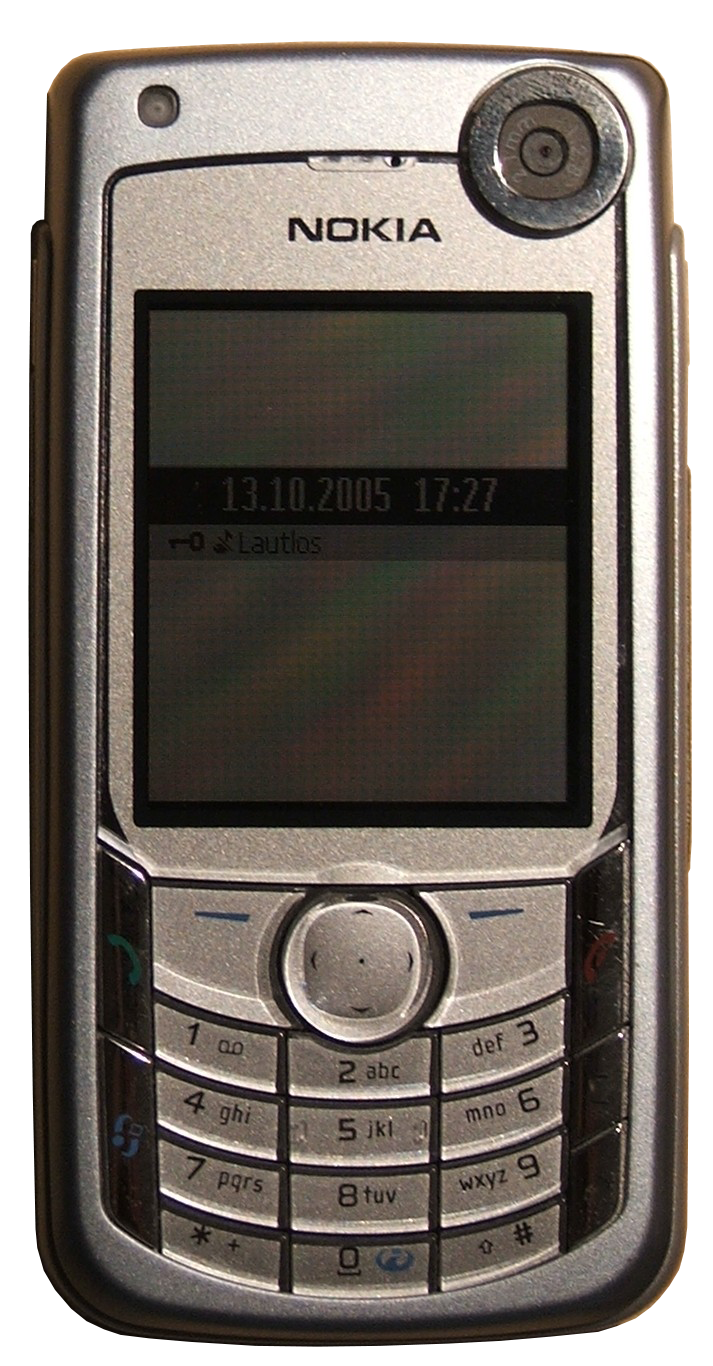
\includegraphics[height=0.23\textheight]{figure/xg/nokia_6680.png}
  \end{columns}
\end{frame}

\begin{frame}{4G made buffering feel like a personal insult}
  \begin{columns}[T,onlytextwidth]
    \column{0.47\textwidth}
      \centering
      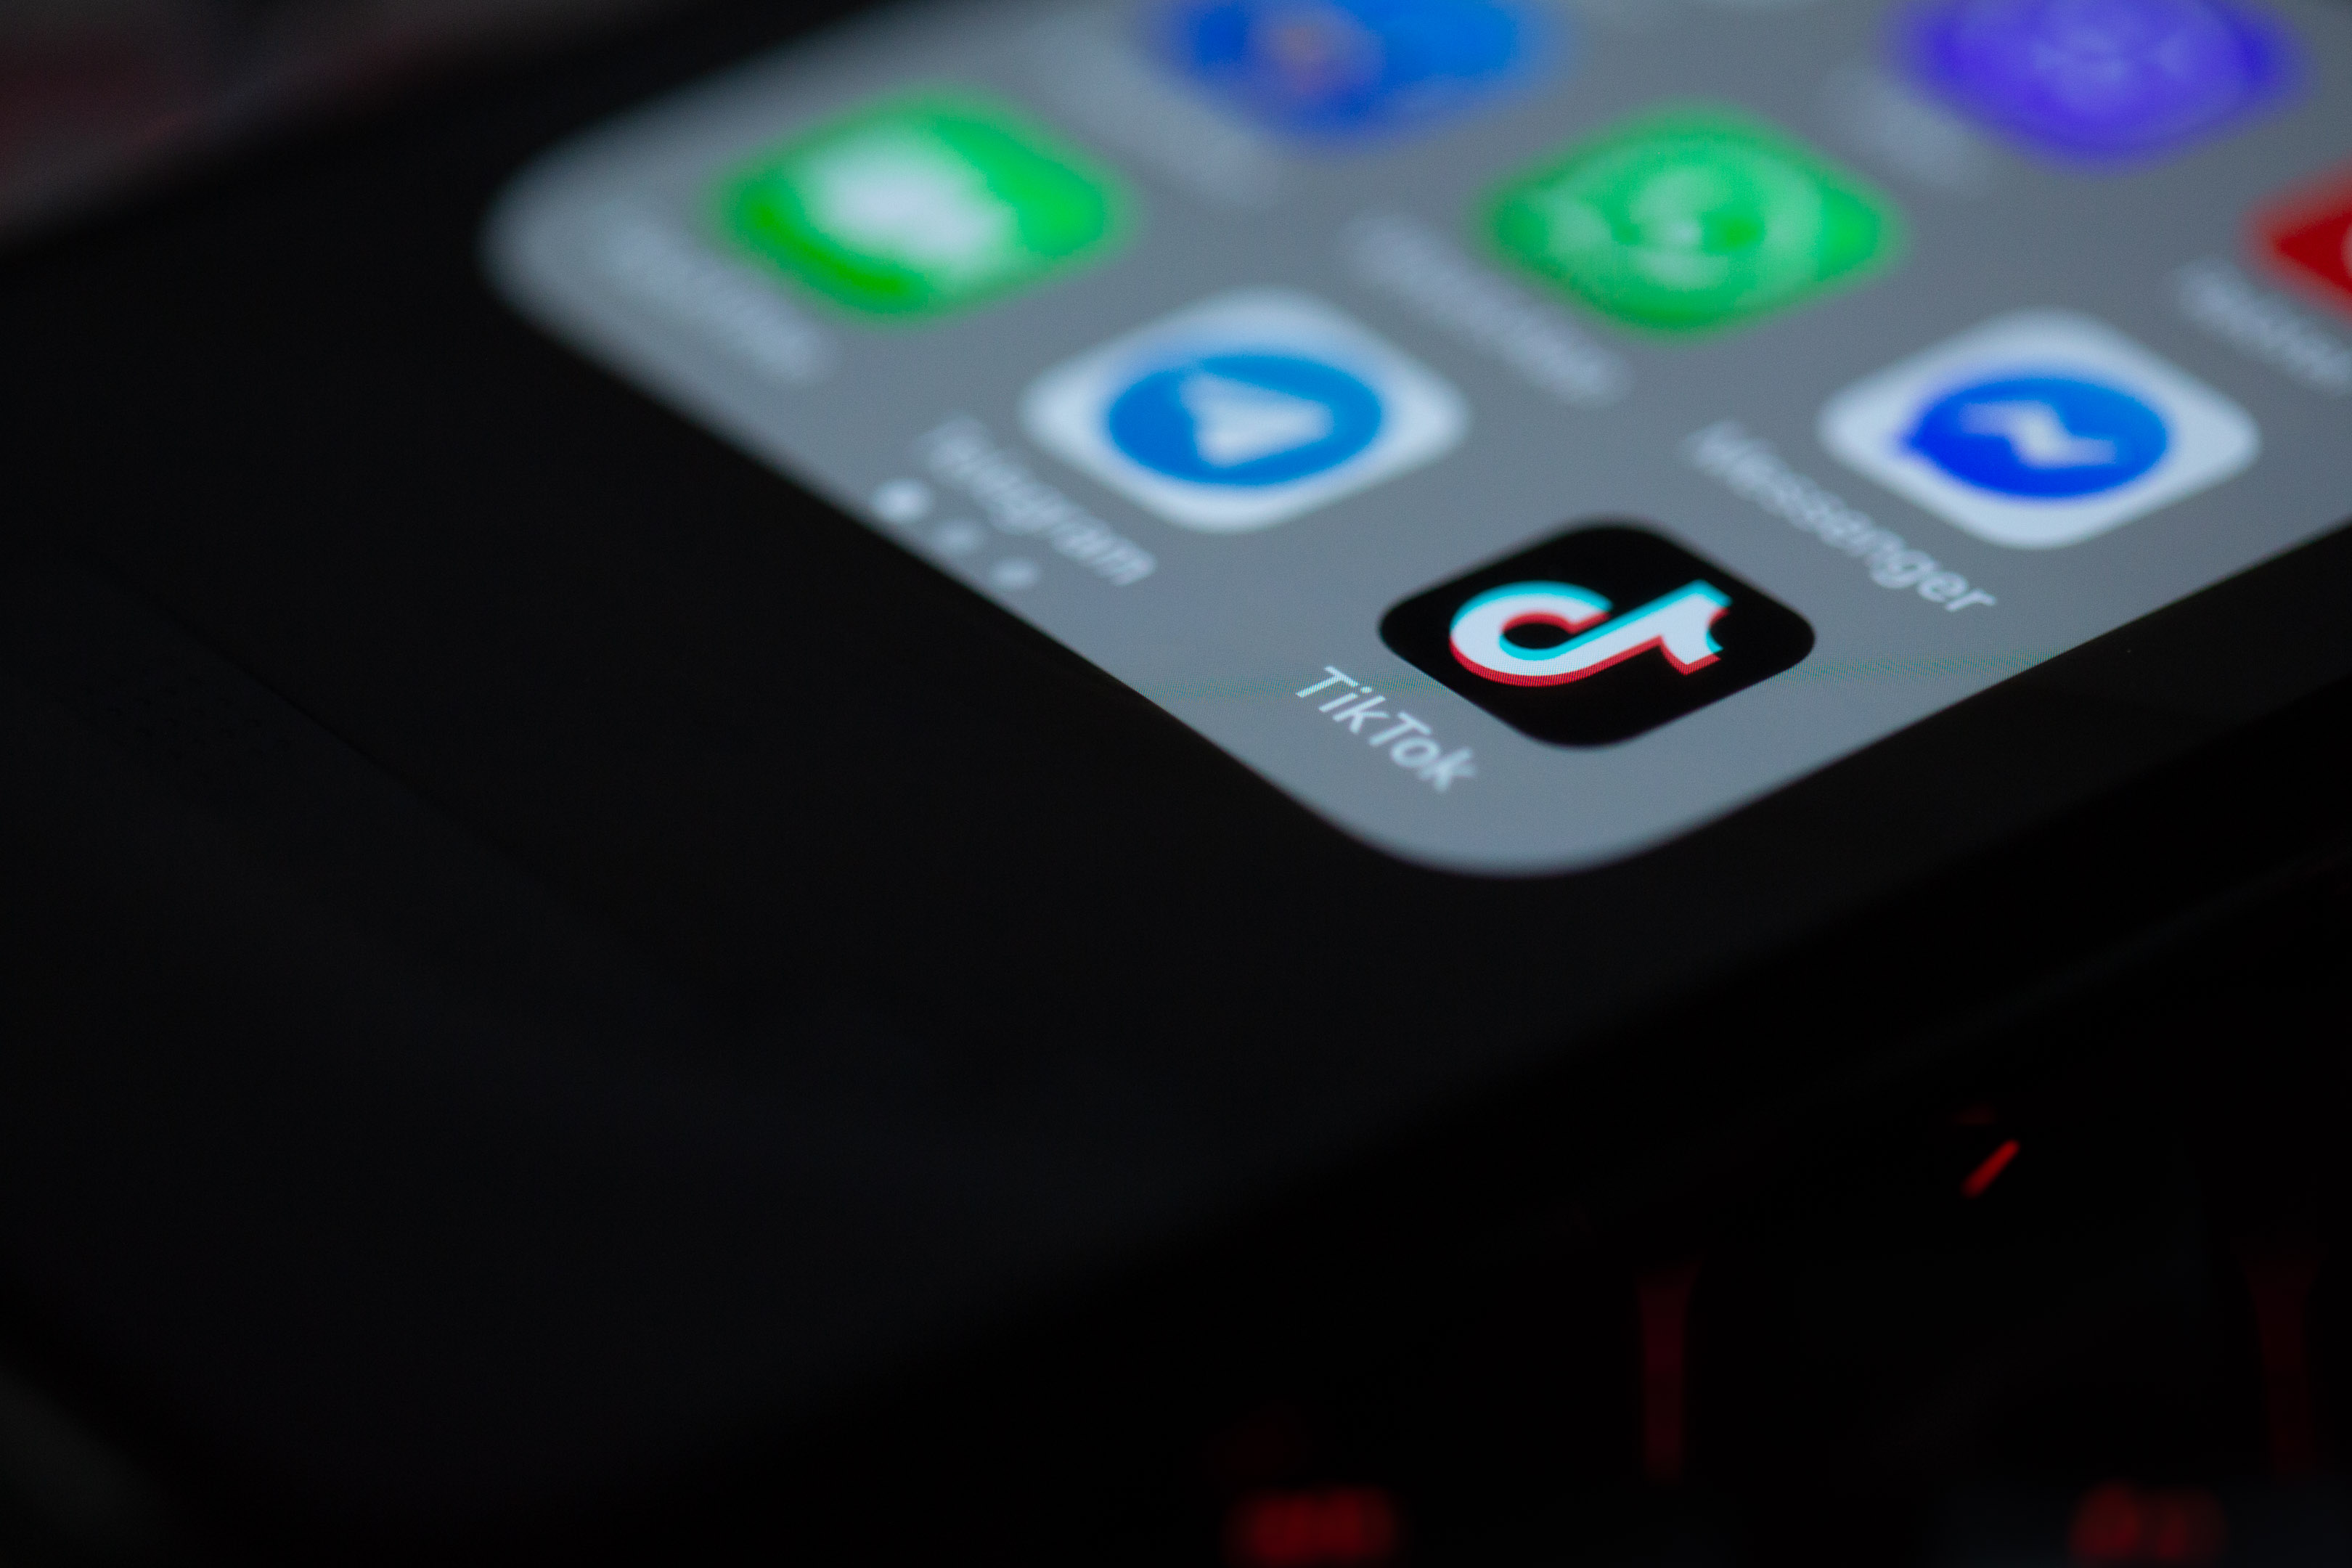
\includegraphics[width=\linewidth]{figure/xg/4g_tiktok_app.jpg}
      \source{https://commons.wikimedia.org/wiki/File:TikTok_app.jpg}{TikTok app on phone}
    \column{0.49\textwidth}
      \large\textbf{Broadband became the default.}
      \normalsize
      \begin{itemize}
        \item Streaming and short video
        \item Maps, ride sharing, live apps
        \item Voice moved toward IP with VoLTE
      \end{itemize}

      \takeaway{4G did not invent video. It made mobile video routine.}
  \end{columns}
\end{frame}

% Video cue (45 s): use the opening comparison. Play 0:20--1:05.
% https://www.youtube.com/watch?v=ik15HVNzJVg
% Forum prompts are anecdotes, not performance evidence.
\begin{frame}{The 5G icon can lie by omission}
  \begin{columns}[T,onlytextwidth]
    \column{0.52\textwidth}
      \centering
      \href{https://www.youtube.com/watch?v=ik15HVNzJVg}{%
        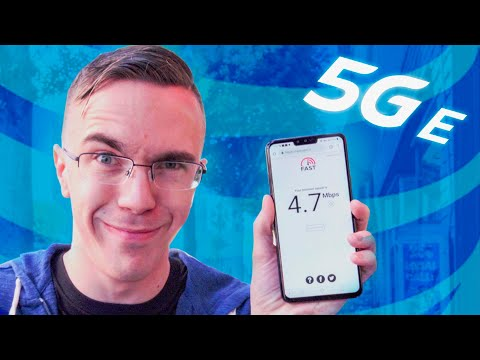
\includegraphics[width=\linewidth]{figure/xg/video_fake5g.jpg}}
      \source{https://www.youtube.com/watch?v=ik15HVNzJVg}{Trying AT\&T's ``5G E'' (YouTube)}
    \column{0.48\textwidth}
      \large\textit{``Why is LTE faster than 5G here?''}
      \source{https://www.reddit.com/r/verizon/comments/1qou5p5/lte/}{Paraphrased user question, 2026}

      \normalsize
      \begin{itemize}
        \item The icon mainly reflects radio access and branding.
        \item Coverage, spectrum, congestion, and deployment mode matter.
        \item A 5G radio can still depend on a 4G core.
      \end{itemize}
  \end{columns}
\end{frame}
